\section{次梯度方法}
\label{sec:ns-subgradient}

有了次梯度，最直接的算法是把梯度下降里的梯度换掉。接下来要弄清：这样换了之后，每一步还是不是在下山？如果不是，靠什么保证有限步之后的目标差可以控制？

\paragraph{主要思想}
设$f:\mathbb{R}^n\to\mathbb{R}$是凸函数，每次可以读取一个函数值和一个次梯度。这种只给函数值和次梯度的读取方式常称为黑箱。\term{次梯度法}（subgradient method）的迭代是
\begin{equation}
 \bm{x}^{(t+1)}=\bm{x}^{(t)}-\alpha^{(t)}\bm{g}^{(t)},\qquad\bm{g}^{(t)}\in\partial f(\bm{x}^{(t)}).
 \label{eq:ns-subgradient-update}
\end{equation}

这里$\bm{g}^{(t)}$的记号沿用了梯度的缩写，表示读到的那一个次梯度。

先看第一个差别：$-\bm{g}^{(t)}$不一定是下降方向。取菱形目标$f(\bm{x})=\lvert x_1\rvert+2\lvert x_2\rvert$，当前点$\bm{x}=(1,0)$，$f(\bm{x})=1$。由上节的计算，$\bm{g}=(1,2)$是一个次梯度。沿$-\bm{g}$走$\alpha$：
\[
 \bm{x}^{+}=(1-\alpha,\,-2\alpha),\qquad f(\bm{x}^{+})=1-\alpha+4\alpha=1+3\alpha.
\]

无论$\alpha>0$多小，目标都上升。第二分量离开零点付出的代价$4\alpha$超过了第一分量的收益。第~\ref{chap:smooth-foundations}章的下降引理在这里完全不成立，线搜索也无从进行：沿这个方向根本没有更低的点。

但走这一步并不是白走。到最优解$\bm{x}^\star=\bm{0}$的距离的平方变成
\[
 (1-\alpha)^2+4\alpha^2=1-2\alpha+5\alpha^2,
\]
当$\alpha<\tfrac25$时比$1$小。目标上升了，到解的距离却缩短了，图~\ref{fig:ns-not-descent}画出了这个现象。

\begin{BookInlineFigure}
  \centering
  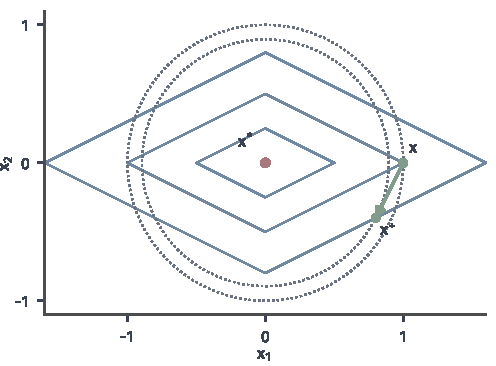
\includegraphics[width=84mm]{figures/05-optimization/03-nonsmooth-optimization/matplotlib/ns-not-descent/figure.pdf}
  \caption{次梯度步不是下降步。蓝线是菱形目标的等高线，由内到外对应$f=0.5,1,1.6$。从$\bm{x}=(1,0)$沿$-\bm{g}=-(1,2)$走$\alpha=0.2$到$\bm{x}^{+}=(0.8,-0.4)$，点越过了$f=1$的等高线，目标升到$1.6$。两个灰色点线圆以$\bm{x}^\star$（红点）为心，新点在内圆上，到解的距离从$1$降到约$0.894$。}
  \label{fig:ns-not-descent}
\end{BookInlineFigure}

原因在支撑不等式~\eqref{eq:ns-subgradient}。取$\bm{y}=\bm{x}^\star$并移项，得到
\begin{equation}
 \langle\bm{g}^{(t)},\bm{x}^{(t)}-\bm{x}^\star\rangle\geq f(\bm{x}^{(t)})-f^\star\geq0.
 \label{eq:ns-subgradient-angle}
\end{equation}

所以$-\bm{g}^{(t)}$与“指向解的方向”$\bm{x}^\star-\bm{x}^{(t)}$夹角不超过直角，目标差越大，这个内积越大。次梯度不保证等高线向内，只保证指向解的那一侧。下面的分析就用距离而不是目标值作为进展的度量。

\paragraph{计算过程}
用菱形目标$f(\bm{x})=\lvert x_1\rvert+2\lvert x_2\rvert$作例子。

\needspace{6\baselineskip}
\paragraph{变量}
\begin{itemize}
 \item $\bm{x}^{(t)}\in\mathbb{R}^n$：当前点；例中$n=2$。
 \item $\bm{g}^{(t)}$：读到的一个次梯度；例中约定把$\operatorname{sign}(0)$取成$+1$，即$\bm{g}=(\pm1,\pm2)$，这样$G=\sqrt5$。
 \item $\alpha^{(t)}$：步长；例中先用固定的$\alpha=0.3$。
 \item $f_{\mathrm{best}}$与$\bm{x}_{\mathrm{best}}$：目前最好的值和点。
\end{itemize}

\paragraph{初始化}
选起点$\bm{x}^{(0)}$，令$f_{\mathrm{best}}=f(\bm{x}^{(0)})$。例中$\bm{x}^{(0)}=(1,1)$，$f_{\mathrm{best}}=3$，到解的距离$R=\sqrt2$。

\needspace{6\baselineskip}
\paragraph{每轮更新}
\begin{enumerate}
 \item 读取$\bm{g}^{(t)}\in\partial f(\bm{x}^{(t)})$。例中第一轮$\bm{g}^{(0)}=(1,2)$。
 \item 由式~\eqref{eq:ns-subgradient-update}计算新点。例中第一轮
 \[
  \bm{x}^{(1)}=(1,1)-0.3\,(1,2)=(0.7,0.4).
 \]
 \item 计算$f(\bm{x}^{(t+1)})$，若比$f_{\mathrm{best}}$小就更新。例中$f(\bm{x}^{(1)})=1.5$，$f_{\mathrm{best}}=1.5$。
\end{enumerate}

后续各轮的结果如下，$\bm{g}^{(t)}$按当前点的符号取得：
\[
 \begin{aligned}
 \bm{x}^{(2)}&=(0.7,0.4)-0.3\,(1,2)=(0.4,-0.2), & f&=0.8,\\
 \bm{x}^{(3)}&=(0.4,-0.2)-0.3\,(1,-2)=(0.1,0.4), & f&=0.9,\\
 \bm{x}^{(4)}&=(0.1,0.4)-0.3\,(1,2)=(-0.2,-0.2), & f&=0.6,\\
 \bm{x}^{(5)}&=(-0.2,-0.2)-0.3\,(-1,-2)=(0.1,0.4), & f&=0.9.
 \end{aligned}
\]

第三轮目标从$0.8$升到$0.9$，第五轮回到了$\bm{x}^{(3)}$，此后在$(0.1,0.4)$和$(-0.2,-0.2)$之间循环。这里没有收敛，$f_{\mathrm{best}}$停在$0.6$。迭代到预定的步数$T$结束，或在已知下界时目标差足够小时结束。最终得到的不是最后一个点，而是$\bm{x}_{\mathrm{best}}=(-0.2,-0.2)$。 图~\ref{fig:ns-subgrad-cycle}画出了路径与目标值。

\begin{BookInlineFigure}
  \centering
  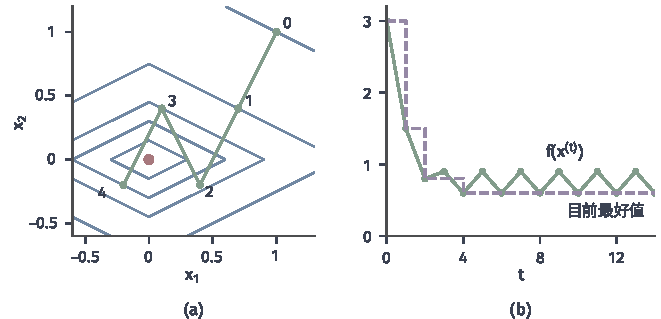
\includegraphics[width=112mm]{figures/05-optimization/03-nonsmooth-optimization/matplotlib/ns-subgrad-cycle/figure.pdf}
  \caption{固定步长$\alpha=0.3$的次梯度法。(a)菱形目标的等高线上前$5$步的路径（绿色），数字是迭代编号，最后两点形成循环。(b)绿线是目标值$f(\bm{x}^{(t)})$，反复升降；紫色虚线是目前最好值，在$0.6$处不再改善。}
  \label{fig:ns-subgrad-cycle}
\end{BookInlineFigure}

\paragraph{距离的递推}
把更新代入距离的平方并展开：
\[
 \lVert\bm{x}^{(t+1)}-\bm{x}^\star\rVert_2^2
 =\lVert\bm{x}^{(t)}-\bm{x}^\star\rVert_2^2
 -2\alpha^{(t)}\langle\bm{g}^{(t)},\bm{x}^{(t)}-\bm{x}^\star\rangle
 +(\alpha^{(t)})^2\lVert\bm{g}^{(t)}\rVert_2^2.
\]

由式~\eqref{eq:ns-subgradient-angle}替换中间一项，得到
\begin{equation}
 \lVert\bm{x}^{(t+1)}-\bm{x}^\star\rVert_2^2
 \leq\lVert\bm{x}^{(t)}-\bm{x}^\star\rVert_2^2
 -2\alpha^{(t)}\bigl(f(\bm{x}^{(t)})-f^\star\bigr)
 +(\alpha^{(t)})^2\lVert\bm{g}^{(t)}\rVert_2^2.
 \label{eq:ns-distance-recursion}
\end{equation}

式~\eqref{eq:ns-distance-recursion}中，目标差是“推进”，步长平方乘次梯度范数是“偏离”。步长小的时候偏离是二阶量，推进是一阶量，所以只要目标差还不小，距离就会缩短。目标差趋近于零时偏离占上风，迭代在解附近抖动，这决定了步长必须逐渐减小。

\begin{theorem}[次梯度法的目标差界]
\label{thm:ns-subgradient-rate}
设$f:\mathbb{R}^n\to\mathbb{R}$是凸函数，最优解$\bm{x}^\star$存在，所有读到的次梯度满足$\lVert\bm{g}^{(t)}\rVert_2\leq G$，$\lVert\bm{x}^{(0)}-\bm{x}^\star\rVert_2\leq R$。按式~\eqref{eq:ns-subgradient-update}迭代$T$步，记
\begin{equation}
 \bar{\bm{x}}^{(T)}=\frac{\sum_{t=0}^{T-1}\alpha^{(t)}\bm{x}^{(t)}}{\sum_{t=0}^{T-1}\alpha^{(t)}},\qquad
 f_{\mathrm{best}}^{(T)}=\min_{0\leq t<T}f(\bm{x}^{(t)}),
 \label{eq:ns-subgradient-outputs}
\end{equation}
则两者都满足
\begin{equation}
 \max\bigl\{f(\bar{\bm{x}}^{(T)}),\,f_{\mathrm{best}}^{(T)}\bigr\}-f^\star
 \leq\frac{R^2+G^2\sum_{t=0}^{T-1}(\alpha^{(t)})^2}{2\sum_{t=0}^{T-1}\alpha^{(t)}}.
 \label{eq:ns-subgradient-bound}
\end{equation}
特别地，预先确定$T$并取固定步长$\alpha^{(t)}=R/(G\sqrt{T})$时，上界为
\begin{equation}
 \frac{RG}{\sqrt{T}}.
 \label{eq:ns-subgradient-rate}
\end{equation}
\end{theorem}

\begin{proof}
把式~\eqref{eq:ns-distance-recursion}对$t=0,\ldots,T-1$相加，左右的距离项错项相消，只剩首尾：
\[
 \lVert\bm{x}^{(T)}-\bm{x}^\star\rVert_2^2\leq R^2-2\sum_{t=0}^{T-1}\alpha^{(t)}\bigl(f(\bm{x}^{(t)})-f^\star\bigr)+G^2\sum_{t=0}^{T-1}(\alpha^{(t)})^2.
\]

左端非负，移项后得到
\[
 2\sum_{t=0}^{T-1}\alpha^{(t)}\bigl(f(\bm{x}^{(t)})-f^\star\bigr)\leq R^2+G^2\sum_{t=0}^{T-1}(\alpha^{(t)})^2.
\]

最好值的目标差不超过各项目标差的$\alpha^{(t)}$加权平均。平均点由Jensen不等式（凸函数在加权平均点的值不超过函数值的同一加权平均，这由凸函数的定义对权重个数归纳得到）也满足
\[
 f(\bar{\bm{x}}^{(T)})-f^\star\leq\frac{\sum_t\alpha^{(t)}\bigl(f(\bm{x}^{(t)})-f^\star\bigr)}{\sum_t\alpha^{(t)}}.
\]
两者除以$2\sum_t\alpha^{(t)}$，就是式~\eqref{eq:ns-subgradient-bound}。

取$\alpha^{(t)}=\alpha$时，右端是$(R^2+TG^2\alpha^2)/(2T\alpha)$，关于$\alpha$在$\alpha=R/(G\sqrt{T})$处最小，代入即得式~\eqref{eq:ns-subgradient-rate}。
\end{proof}

定理的条件都用上了。凸性给出式~\eqref{eq:ns-subgradient-angle}；次梯度有界使偏离项可控，Lipschitz连续的函数自动满足这一条，常数$G$就是Lipschitz常数；最优解存在，$R$才有意义。结论说的是平均点或最好点，最后一点$\bm{x}^{(T)}$不在其中。

回到上面的小例子，式~\eqref{eq:ns-subgradient-bound}对$f_{\mathrm{best}}$的预言是$T=5$时不超过
\[
 \frac{2+5\cdot5\cdot0.09}{2\cdot5\cdot0.3}=\frac{4.25}{3}\approx1.417,
\]
实际的$f_{\mathrm{best}}=0.6$。当$T\to\infty$时，这个界趋于$G^2\alpha/2=0.75$，固定步长的上界也只能给到一个邻域。

\paragraph{步长规则}
式~\eqref{eq:ns-subgradient-bound}告诉我们要什么：分子增长比分母慢，这需要$\sum_t\alpha^{(t)}=\infty$，同时$\alpha^{(t)}\to0$使平方和相对于和可以忽略。满足这两条的递减步长，如$\alpha^{(t)}=c/\sqrt{t+1}$，右端趋于$0$。它们不需要预先知道$T$，代价是界多出一个对数因子。

若最优值$f^\star$已知，可以直接优化式~\eqref{eq:ns-distance-recursion}的右端。关于$\alpha^{(t)}$求最小，得到\term{Polyak步长}（Polyak step size）：
\begin{equation}
 \alpha^{(t)}=\frac{f(\bm{x}^{(t)})-f^\star}{\lVert\bm{g}^{(t)}\rVert_2^2}.
 \label{eq:ns-polyak-step}
\end{equation}

把它代回式~\eqref{eq:ns-distance-recursion}，得到每步距离的减少量：
\[
 \lVert\bm{x}^{(t+1)}-\bm{x}^\star\rVert_2^2\leq\lVert\bm{x}^{(t)}-\bm{x}^\star\rVert_2^2-\frac{(f(\bm{x}^{(t)})-f^\star)^2}{\lVert\bm{g}^{(t)}\rVert_2^2}.
\]

相加后同样得到$\min_{t<T}f(\bm{x}^{(t)})-f^\star\leq RG/\sqrt{T}$，不用事先知道$R$、$G$和$T$，但要知道$f^\star$，这在部分问题上成立，例如已知最优值为零的可行性问题。例中从$(1,0)$、$\bm{g}=(1,2)$出发，$\alpha=1/5$，点变成$(0.8,-0.4)$，就是图~\ref{fig:ns-not-descent}的那一步。

\paragraph{输出什么}
目前最好点需要每轮多算一次函数值，好处是保证单调；加权平均点不用算函数值，只需累加向量。最后一点没有上述保证。图~\ref{fig:ns-subgrad-rates}用递减步长$\alpha^{(t)}=R/(G\sqrt{t+1})$比较三者，横轴是步数，三条曲线都在上界之下，最后一点在一条带内不断跳动，目前最好点和加权平均点则是稳定的。

\begin{BookInlineFigure}
  \centering
  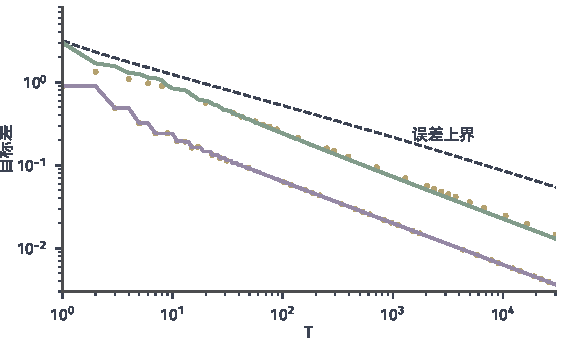
\includegraphics[width=96mm]{figures/05-optimization/03-nonsmooth-optimization/matplotlib/ns-subgrad-rates/figure.pdf}
  \caption{次梯度法的三种输出（双对数坐标）。目标是菱形目标，$\bm{x}^{(0)}=(1,1)$，步长$\alpha^{(t)}=R/(G\sqrt{t+1})$。黄点是采样的最后点目标差，它随$t$的奇偶在一条带内跳动；绿线是加权平均点；紫线是目前最好点；黑色虚线是式~\eqref{eq:ns-subgradient-bound}的上界。}
  \label{fig:ns-subgrad-rates}
\end{BookInlineFigure}

\paragraph{为什么慢，以及慢到什么程度}
要达到目标差$\varepsilon$，由式~\eqref{eq:ns-subgradient-rate}需要$T\geq R^2G^2/\varepsilon^2$步。精度提高十倍，步数增加一百倍。梯度下降在光滑凸目标上的步数是$O(1/\varepsilon)$，这里慢了一个量级。

这不是分析得不够细。只通过函数值和次梯度了解目标的方法，在维数足够大时存在最坏的函数，使任何这类方法在前若干步的目标差都不低于$RG/(2(1+\sqrt{T}))$这样的量级，所以$RG/\sqrt{T}$在黑箱模型下不能本质改进。这个下界的证明需要构造一族对抗性函数，篇幅较长，这里只用它的含义：要比$1/\sqrt{T}$更快，就不能只靠黑箱，必须用上目标的结构。

次梯度法的优势在于通用和便宜：每步只要一个次梯度，存储一个向量，不需要光滑性和邻近映射。后面几节的方法都要求多知道一些东西。
